\documentclass[a4paper]{article}

\usepackage[
    % fancytheorems, 
    % fancyproofs, 
    % noindent, 
    nokoma
]{adam}

% \documentclass[a4paper]{scrartcl}

% \usepackage[
%     fancytheorems, 
%     fancyproofs, 
%     noindent, 
% ]{adam}

\title{Geometry}
\author{Adam Kelly (\texttt{ak2316@cam.ac.uk})}
\date{\today}

\allowdisplaybreaks

\begin{document}

\maketitle

% This is a short description of the course. It should give a little flavour of what the course is about, and what will be roughly covered in the notes.

This article constitutes my notes for the `Geometry' course, held in Lent 2022 at Cambridge. These notes are \emph{not a transcription of the lectures}, and differ significantly in quite a few areas. 
In particular, many of the examples given in lectures (including the extended ones) are \emph{excluded}, and instead just the outer structure of the subject has been left.
It is assumed that the reader is very familiar with the content from the `Analysis and Topology' course.

Note that the section of the course on Hyperbolic geometry has been omitted
%Still, all lectured material should be covered.
%In 

\tableofcontents

\section{Surfaces}

\subsection{Topological Surfaces}

The idea of a surface is to try and generalize `the plane' to an object where everything isn't necessarily `flat', as one might imagine with $\R^2$. 
For example, we can take some surfaces as drawn below.

\begin{center}
    

\tikzset{every picture/.style={line width=0.75pt}} %set default line width to 0.75pt        

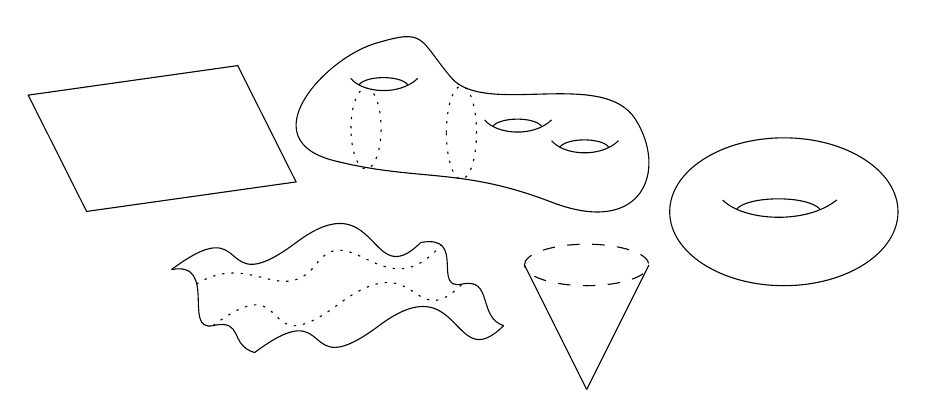
\begin{tikzpicture}[x=0.75pt,y=0.75pt,yscale=-1,xscale=1]
%uncomment if require: \path (0,202); %set diagram left start at 0, and has height of 202

%Curve Lines [id:da5236115066615021] 
\draw    (375.49,78.68) .. controls (385.11,88.65) and (415.36,90.93) .. (430.49,78.68) ;
%Curve Lines [id:da7101991261257758] 
\draw    (422.24,82.95) .. controls (415.91,76.4) and (388.14,76.68) .. (382.36,82.95) ;
%Shape: Ellipse [id:dp9157295048532674] 
\draw   (350,84.38) .. controls (350,64.7) and (374.62,48.75) .. (405,48.75) .. controls (435.38,48.75) and (460,64.7) .. (460,84.38) .. controls (460,104.05) and (435.38,120) .. (405,120) .. controls (374.62,120) and (350,104.05) .. (350,84.38) -- cycle ;
%Shape: Polygon Curved [id:ds6159505592009495] 
\draw   (208.2,3.25) .. controls (232.62,-4.05) and (228.75,0.75) .. (244.72,19.75) .. controls (260.69,38.75) and (317.8,15.15) .. (333.44,39.75) .. controls (349.09,64.35) and (337.15,96.75) .. (293.11,79.75) .. controls (249.08,62.75) and (228.75,69.95) .. (188.26,59.75) .. controls (147.77,49.55) and (183.78,10.55) .. (208.2,3.25) -- cycle ;
%Curve Lines [id:da5470586253636169] 
\draw    (196.33,20.12) .. controls (201.97,27.12) and (219.72,28.72) .. (228.59,20.12) ;
%Curve Lines [id:da010111340882360542] 
\draw    (223.75,23.12) .. controls (220.04,18.52) and (203.75,18.72) .. (200.36,23.12) ;
%Curve Lines [id:da5844912655809358] 
\draw    (260.85,40.12) .. controls (266.5,47.12) and (284.24,48.72) .. (293.11,40.12) ;
%Curve Lines [id:da11520475628245719] 
\draw    (288.28,43.12) .. controls (284.57,38.52) and (268.27,38.72) .. (264.88,43.12) ;
%Curve Lines [id:da20029327068385938] 
\draw    (293.11,50.12) .. controls (298.76,57.12) and (316.5,58.72) .. (325.38,50.12) ;
%Curve Lines [id:da040106671156743934] 
\draw    (320.54,53.12) .. controls (316.83,48.52) and (300.53,48.72) .. (297.15,53.12) ;
%Shape: Parallelogram [id:dp5212701228907126] 
\draw   (40.94,28.18) -- (141.87,13.96) -- (170,70) -- (69.07,84.22) -- cycle ;
%Curve Lines [id:da9139712577644594] 
\draw    (110,112.22) .. controls (150,82.22) and (130,129.22) .. (170,99.22) .. controls (210,69.22) and (205,124.22) .. (230,99.22) ;
%Curve Lines [id:da7132152828416398] 
\draw    (150,152.22) .. controls (190,122.22) and (170,169.22) .. (210,139.22) .. controls (250,109.22) and (245,164.22) .. (270,139.22) ;
%Curve Lines [id:da7754830305851486] 
\draw    (110,112.22) .. controls (132.5,107.97) and (115,142.47) .. (130,139.22) .. controls (145,135.97) and (137.5,148.47) .. (150,152.22) ;
%Curve Lines [id:da594486777960795] 
\draw    (230,99.22) .. controls (252.5,94.97) and (235,122.47) .. (250,119.22) .. controls (265,115.97) and (257.5,135.47) .. (270,139.22) ;
%Curve Lines [id:da5052126741414245] 
\draw  [dash pattern={on 0.84pt off 2.51pt}]  (130,139.22) .. controls (170,109.22) and (150,159.22) .. (190,129.22) .. controls (230,99.22) and (225,144.22) .. (250,119.22) ;
%Curve Lines [id:da3191700592357998] 
\draw  [dash pattern={on 0.84pt off 2.51pt}]  (122,119.22) .. controls (148,102.97) and (163.5,130.97) .. (180,109.22) .. controls (196.5,87.47) and (213.5,131.47) .. (240,100.22) ;
%Shape: Ellipse [id:dp5455375672721312] 
\draw  [dash pattern={on 0.84pt off 2.51pt}] (242.41,46.25) .. controls (242.41,33.82) and (245.66,23.75) .. (249.67,23.75) .. controls (253.67,23.75) and (256.92,33.82) .. (256.92,46.25) .. controls (256.92,58.67) and (253.67,68.75) .. (249.67,68.75) .. controls (245.66,68.75) and (242.41,58.67) .. (242.41,46.25) -- cycle ;
%Shape: Ellipse [id:dp7528987294411815] 
\draw  [dash pattern={on 0.84pt off 2.51pt}] (196.43,44.25) .. controls (196.43,33.48) and (199.68,24.75) .. (203.69,24.75) .. controls (207.7,24.75) and (210.95,33.48) .. (210.95,44.25) .. controls (210.95,55.02) and (207.7,63.75) .. (203.69,63.75) .. controls (199.68,63.75) and (196.43,55.02) .. (196.43,44.25) -- cycle ;
%Shape: Ellipse [id:dp915900620670441] 
\draw  [dash pattern={on 4.5pt off 4.5pt}] (280,110) .. controls (280,104.48) and (293.43,100) .. (310,100) .. controls (326.57,100) and (340,104.48) .. (340,110) .. controls (340,115.52) and (326.57,120) .. (310,120) .. controls (293.43,120) and (280,115.52) .. (280,110) -- cycle ;
%Straight Lines [id:da8069294757540748] 
\draw    (280,110) -- (310,170) ;
%Straight Lines [id:da5092407774777901] 
\draw    (340,110) -- (310,170) ;




\end{tikzpicture}

\end{center}

We really care about surfaces that have two dimensions, in that a small region around each point in the surface looks just like a plane. It's these ideas that manifest into our basic notion of a \emph{topological surface}.

\begin{definition}[Topological Surface]
    A \vocab{topological surface} is a topological space $\Sigma$ such that
    \begin{enumerate}[label=(\roman*)]
        \item For each $p \in \Sigma$, there's an open neighborhood $U \subset \Sigma$ with $p \in U$ such that $U$ is homeomorphic to $\R^2$ with its usual Euclidean topology.
        \item $\Sigma$ is Hausdorff and second countable.
    \end{enumerate}
\end{definition}

Here, the true nature of the definition is in (i), that our space looks locally like $\R^2$. The other part (ii) of the definition is really just there to make technical things work out properly later on. 

With neighborhoods around each point looking like $\R^2$, we can sensibly imagine that one could locally put a coordinate system on such neighborhoods, one coming from the homeomorphism to $\R^2$. This motivates the definition of a \emph{chart} on a topological surface.

\begin{center}
    

\tikzset{every picture/.style={line width=0.75pt}} %set default line width to 0.75pt        

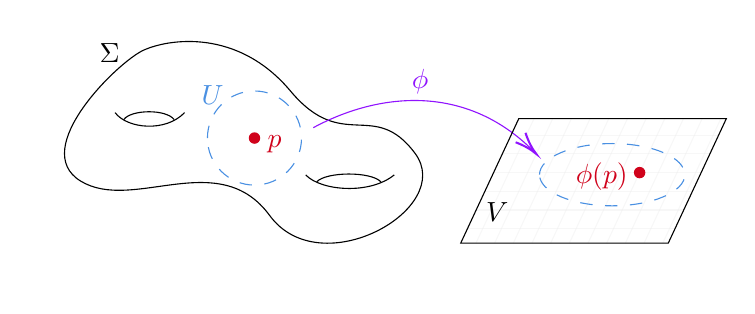
\begin{tikzpicture}[x=0.75pt,y=0.75pt,yscale=-1,xscale=1]
%uncomment if require: \path (0,315); %set diagram left start at 0, and has height of 315

%Shape: Grid [id:dp2824817026261346] 
\draw  [draw opacity=0] (409.35,113.32) -- (510,113.32) -- (482.02,173.32) -- (381.37,173.32) -- cycle ; \draw  [color={rgb, 255:red, 235; green, 235; blue, 235 }  ,draw opacity=0.39 ] (417.35,113.32) -- (389.37,173.32)(426.35,113.32) -- (398.37,173.32)(435.35,113.32) -- (407.37,173.32)(444.35,113.32) -- (416.37,173.32)(453.35,113.32) -- (425.37,173.32)(462.35,113.32) -- (434.37,173.32)(471.35,113.32) -- (443.37,173.32)(480.35,113.32) -- (452.37,173.32)(489.35,113.32) -- (461.37,173.32)(498.35,113.32) -- (470.37,173.32)(507.35,113.32) -- (479.37,173.32) ; \draw  [color={rgb, 255:red, 235; green, 235; blue, 235 }  ,draw opacity=0.39 ] (405.62,121.32) -- (506.27,121.32)(401.43,130.32) -- (502.07,130.32)(397.23,139.32) -- (497.88,139.32)(393.03,148.32) -- (493.68,148.32)(388.84,157.32) -- (489.48,157.32)(384.64,166.32) -- (485.29,166.32) ; \draw  [color={rgb, 255:red, 235; green, 235; blue, 235 }  ,draw opacity=0.39 ]  ;
%Shape: Polygon Curved [id:ds10590282788241523] 
\draw   (229.18,80.36) .. controls (241.44,74.78) and (274.67,69.76) .. (300,100) .. controls (325.33,130.24) and (340.15,103.45) .. (360,130) .. controls (379.85,156.55) and (314.5,193.47) .. (290,160) .. controls (265.5,126.53) and (224.14,158.79) .. (198.9,143.39) .. controls (173.66,128) and (216.93,85.94) .. (229.18,80.36) -- cycle ;
%Curve Lines [id:da5406567027069826] 
\draw    (215.5,110.42) .. controls (221.36,118.23) and (239.79,120.01) .. (249,110.42) ;
%Curve Lines [id:da11605042813104172] 
\draw    (243.97,113.77) .. controls (240.12,108.63) and (223.2,108.86) .. (219.69,113.77) ;
%Curve Lines [id:da8421916068847695] 
\draw    (307.33,140.42) .. controls (314.8,148.23) and (338.27,150.01) .. (350,140.42) ;
%Curve Lines [id:da5979992538827481] 
\draw    (343.6,143.77) .. controls (338.69,138.63) and (317.14,138.86) .. (312.66,143.77) ;
%Shape: Circle [id:dp7284538694447111] 
\draw  [draw opacity=0][fill={rgb, 255:red, 208; green, 2; blue, 27 }  ,fill opacity=1 ] (279.92,122.67) .. controls (279.92,121.15) and (281.15,119.92) .. (282.67,119.92) .. controls (284.19,119.92) and (285.42,121.15) .. (285.42,122.67) .. controls (285.42,124.19) and (284.19,125.42) .. (282.67,125.42) .. controls (281.15,125.42) and (279.92,124.19) .. (279.92,122.67) -- cycle ;
%Shape: Circle [id:dp8388763618077151] 
\draw  [color={rgb, 255:red, 74; green, 144; blue, 226 }  ,draw opacity=1 ][dash pattern={on 4.5pt off 4.5pt}] (260,122.67) .. controls (260,110.15) and (270.15,100) .. (282.67,100) .. controls (295.19,100) and (305.33,110.15) .. (305.33,122.67) .. controls (305.33,135.19) and (295.19,145.33) .. (282.67,145.33) .. controls (270.15,145.33) and (260,135.19) .. (260,122.67) -- cycle ;
%Curve Lines [id:da4312845382129431] 
\draw [color={rgb, 255:red, 144; green, 19; blue, 254 }  ,draw opacity=1 ]   (311,117.68) .. controls (341.69,101.07) and (384.23,95.68) .. (417.42,129.29) ;
\draw [shift={(418.43,130.32)}, rotate = 226.19] [color={rgb, 255:red, 144; green, 19; blue, 254 }  ,draw opacity=1 ][line width=0.75]    (10.93,-3.29) .. controls (6.95,-1.4) and (3.31,-0.3) .. (0,0) .. controls (3.31,0.3) and (6.95,1.4) .. (10.93,3.29)   ;
%Shape: Ellipse [id:dp020561129589376614] 
\draw  [color={rgb, 255:red, 74; green, 144; blue, 226 }  ,draw opacity=1 ][dash pattern={on 4.5pt off 4.5pt}] (420,140.32) .. controls (420,132.04) and (435.67,125.32) .. (455,125.32) .. controls (474.33,125.32) and (490,132.04) .. (490,140.32) .. controls (490,148.61) and (474.33,155.32) .. (455,155.32) .. controls (435.67,155.32) and (420,148.61) .. (420,140.32) -- cycle ;
%Shape: Rectangle [id:dp6823458888863583] 
\draw   (410,113.32) -- (510,113.32) -- (482.02,173.32) -- (382.02,173.32) -- cycle ;
%Shape: Circle [id:dp01371884157878056] 
\draw  [draw opacity=0][fill={rgb, 255:red, 208; green, 2; blue, 27 }  ,fill opacity=1 ] (465.48,139.32) .. controls (465.48,137.8) and (466.71,136.57) .. (468.23,136.57) .. controls (469.75,136.57) and (470.98,137.8) .. (470.98,139.32) .. controls (470.98,140.84) and (469.75,142.07) .. (468.23,142.07) .. controls (466.71,142.07) and (465.48,140.84) .. (465.48,139.32) -- cycle ;

% Text Node
\draw (287.75,125.75) node [anchor=west] [inner sep=0.75pt]  [color={rgb, 255:red, 208; green, 2; blue, 27 }  ,opacity=1 ]  {$p$};
% Text Node
\draw (269,107.6) node [anchor=south east] [inner sep=0.75pt]  [color={rgb, 255:red, 74; green, 144; blue, 226 }  ,opacity=1 ]  {$U$};
% Text Node
\draw (219,87.6) node [anchor=south east] [inner sep=0.75pt]    {$\Sigma $};
% Text Node
\draw (362.5,102.6) node [anchor=south] [inner sep=0.75pt]  [color={rgb, 255:red, 144; green, 19; blue, 254 }  ,opacity=1 ]  {$\phi $};
% Text Node
\draw (393,152.4) node [anchor=north west][inner sep=0.75pt]    {$V$};
% Text Node
\draw (463.75,141.07) node [anchor=east] [inner sep=0.75pt]  [color={rgb, 255:red, 208; green, 2; blue, 27 }  ,opacity=1 ]  {$\phi ( p)$};


\end{tikzpicture}

\end{center}

\begin{definition}[Chart]
    A \vocab{chart} for $\Sigma$ is a pair $(U, \phi)$ where $U \subset \Sigma$ and $\phi: U \rightarrow V \subset \R^2$ is a homomorphism. 
\end{definition}

Charts define `local' coordinate systems for our topological surface, and a collection of charts which can give coordinate systems to points everywhere on the surface is called an \emph{atlas}.

\begin{definition}[Atlas]
    An \vocab{atlas} for $\Sigma$ is a collection of charts $(U_i, \phi_i)$ with $i$ in some index set $I$ such that $\bigcup_{i} U_i = \Sigma$.
\end{definition}

In general, we can reasonably imagine that a single point might be covered by more than one chart. Movement between the charts where they intersect on the surface is specified by \emph{transition maps}.

\begin{definition}[Transition Maps]
    Let $(U_1, \phi_1)$ and $(U_2, \phi_2$ be charts containing a point $p$ on a topological surface $\Sigma$.
    Considering the intersection of $U_1$ and $U_2$, we get a \vocab{transition map} $\phi_1(U \cap U_2) \rightarrow \phi_2(U_1 \cap U_2)$ between the charts, and this is a homeomorphism of open sets in $\R^2$.
\end{definition}

\begin{center}
    

\tikzset{every picture/.style={line width=0.75pt}} %set default line width to 0.75pt        

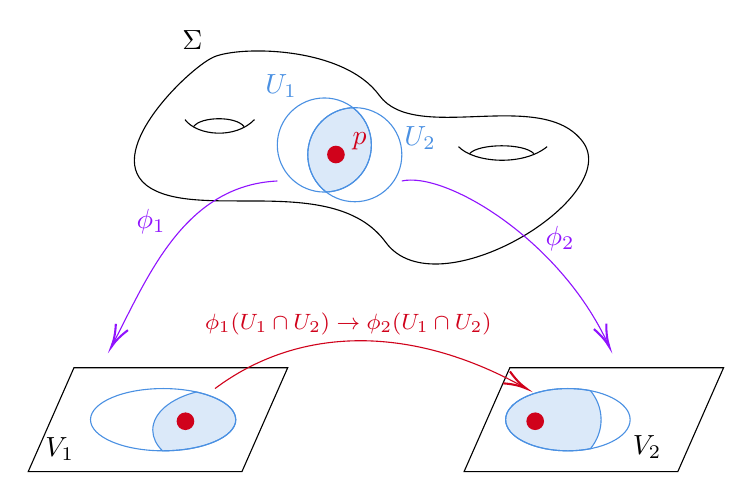
\begin{tikzpicture}[x=0.75pt,y=0.75pt,yscale=-1,xscale=1]
%uncomment if require: \path (0,315); %set diagram left start at 0, and has height of 315

%Shape: Path Data [id:dp019553757401191252] 
\draw  [color={rgb, 255:red, 74; green, 144; blue, 226 }  ,draw opacity=1 ][fill={rgb, 255:red, 74; green, 144; blue, 226 }  ,fill opacity=0.2 ] (240,255) .. controls (240,263.28) and (224.33,270) .. (205,270) .. controls (204.89,270) and (204.79,270) .. (204.68,270) .. controls (201.7,267.06) and (200,263.64) .. (200,260) .. controls (200,251.79) and (208.65,244.74) .. (221.02,241.66) .. controls (232.29,244.15) and (240,249.19) .. (240,255) -- cycle ;
%Shape: Path Data [id:dp24276589649513092] 
\draw  [color={rgb, 255:red, 74; green, 144; blue, 226 }  ,draw opacity=1 ][fill={rgb, 255:red, 74; green, 144; blue, 226 }  ,fill opacity=0.2 ] (400,240) .. controls (403.83,240) and (407.5,240.36) .. (410.87,241.02) .. controls (414.11,245.01) and (416,249.82) .. (416,255) .. controls (416,260.18) and (414.11,264.99) .. (410.87,268.98) .. controls (407.5,269.64) and (403.83,270) .. (400,270) .. controls (383.43,270) and (370,263.28) .. (370,255) .. controls (370,246.72) and (383.43,240) .. (400,240) -- cycle ;
%Shape: Path Data [id:dp09796809086314018] 
\draw  [color={rgb, 255:red, 74; green, 144; blue, 226 }  ,draw opacity=1 ][fill={rgb, 255:red, 74; green, 144; blue, 226 }  ,fill opacity=0.2 ] (305.33,122.67) .. controls (305.33,134.89) and (295.65,144.86) .. (283.53,145.32) .. controls (278.14,141.17) and (274.67,134.66) .. (274.67,127.33) .. controls (274.67,115.11) and (284.35,105.14) .. (296.47,104.68) .. controls (301.86,108.83) and (305.33,115.34) .. (305.33,122.67) -- cycle ;
%Shape: Polygon Curved [id:ds7095918404686692] 
\draw   (229.18,80.36) .. controls (241.44,74.78) and (291.76,74.89) .. (309.16,98.77) .. controls (326.56,122.64) and (387.32,94.53) .. (407.17,121.08) .. controls (427.02,147.63) and (336.76,203.03) .. (312.26,169.56) .. controls (287.76,136.09) and (224.14,158.79) .. (198.9,143.39) .. controls (173.66,128) and (216.93,85.94) .. (229.18,80.36) -- cycle ;
%Curve Lines [id:da18331565679370598] 
\draw    (215.5,110.42) .. controls (221.36,118.23) and (239.79,120.01) .. (249,110.42) ;
%Curve Lines [id:da576658372467886] 
\draw    (243.97,113.77) .. controls (240.12,108.63) and (223.2,108.86) .. (219.69,113.77) ;
%Curve Lines [id:da7636386743100172] 
\draw    (347.33,123.46) .. controls (354.8,131.27) and (378.27,133.05) .. (390,123.46) ;
%Curve Lines [id:da07193806885436627] 
\draw    (383.6,126.8) .. controls (378.69,121.67) and (357.14,121.89) .. (352.66,126.8) ;
%Shape: Circle [id:dp786749563505935] 
\draw  [draw opacity=0][fill={rgb, 255:red, 208; green, 2; blue, 27 }  ,fill opacity=1 ] (284,127.25) .. controls (284,124.9) and (285.9,123) .. (288.25,123) .. controls (290.6,123) and (292.5,124.9) .. (292.5,127.25) .. controls (292.5,129.6) and (290.6,131.5) .. (288.25,131.5) .. controls (285.9,131.5) and (284,129.6) .. (284,127.25) -- cycle ;
%Shape: Circle [id:dp3185974187130436] 
\draw  [color={rgb, 255:red, 74; green, 144; blue, 226 }  ,draw opacity=1 ] (260,122.67) .. controls (260,110.15) and (270.15,100) .. (282.67,100) .. controls (295.19,100) and (305.33,110.15) .. (305.33,122.67) .. controls (305.33,135.19) and (295.19,145.33) .. (282.67,145.33) .. controls (270.15,145.33) and (260,135.19) .. (260,122.67) -- cycle ;
%Shape: Circle [id:dp33857165577509596] 
\draw  [color={rgb, 255:red, 74; green, 144; blue, 226 }  ,draw opacity=1 ] (274.67,127.33) .. controls (274.67,114.81) and (284.81,104.67) .. (297.33,104.67) .. controls (309.85,104.67) and (320,114.81) .. (320,127.33) .. controls (320,139.85) and (309.85,150) .. (297.33,150) .. controls (284.81,150) and (274.67,139.85) .. (274.67,127.33) -- cycle ;
%Shape: Parallelogram [id:dp07551633753566489] 
\draw   (162.02,230) -- (265,230) -- (242.98,280) -- (140,280) -- cycle ;
%Shape: Parallelogram [id:dp931384769198357] 
\draw   (372.02,230) -- (475,230) -- (452.98,280) -- (350,280) -- cycle ;
%Curve Lines [id:da7729008053297273] 
\draw [color={rgb, 255:red, 144; green, 19; blue, 254 }  ,draw opacity=1 ]   (260,140) .. controls (214.69,142.2) and (197.19,187.19) .. (180.75,218.58) ;
\draw [shift={(180,220)}, rotate = 297.93] [color={rgb, 255:red, 144; green, 19; blue, 254 }  ,draw opacity=1 ][line width=0.75]    (10.93,-3.29) .. controls (6.95,-1.4) and (3.31,-0.3) .. (0,0) .. controls (3.31,0.3) and (6.95,1.4) .. (10.93,3.29)   ;
%Curve Lines [id:da685041351732079] 
\draw [color={rgb, 255:red, 144; green, 19; blue, 254 }  ,draw opacity=1 ]   (320,140) .. controls (340.79,135.28) and (395.88,167.9) .. (419.3,218.46) ;
\draw [shift={(420,220)}, rotate = 245.91] [color={rgb, 255:red, 144; green, 19; blue, 254 }  ,draw opacity=1 ][line width=0.75]    (10.93,-3.29) .. controls (6.95,-1.4) and (3.31,-0.3) .. (0,0) .. controls (3.31,0.3) and (6.95,1.4) .. (10.93,3.29)   ;
%Shape: Ellipse [id:dp07767152455305415] 
\draw  [color={rgb, 255:red, 74; green, 144; blue, 226 }  ,draw opacity=1 ] (170,255) .. controls (170,246.72) and (185.67,240) .. (205,240) .. controls (224.33,240) and (240,246.72) .. (240,255) .. controls (240,263.28) and (224.33,270) .. (205,270) .. controls (185.67,270) and (170,263.28) .. (170,255) -- cycle ;
%Shape: Ellipse [id:dp9357255906838657] 
\draw  [color={rgb, 255:red, 74; green, 144; blue, 226 }  ,draw opacity=1 ] (370,255) .. controls (370,246.72) and (383.43,240) .. (400,240) .. controls (416.57,240) and (430,246.72) .. (430,255) .. controls (430,263.28) and (416.57,270) .. (400,270) .. controls (383.43,270) and (370,263.28) .. (370,255) -- cycle ;
%Shape: Circle [id:dp5331273349796806] 
\draw  [draw opacity=0][fill={rgb, 255:red, 208; green, 2; blue, 27 }  ,fill opacity=1 ] (211.5,255.75) .. controls (211.5,253.4) and (213.4,251.5) .. (215.75,251.5) .. controls (218.1,251.5) and (220,253.4) .. (220,255.75) .. controls (220,258.1) and (218.1,260) .. (215.75,260) .. controls (213.4,260) and (211.5,258.1) .. (211.5,255.75) -- cycle ;
%Shape: Circle [id:dp38149586769758015] 
\draw  [draw opacity=0][fill={rgb, 255:red, 208; green, 2; blue, 27 }  ,fill opacity=1 ] (380,255.75) .. controls (380,253.4) and (381.9,251.5) .. (384.25,251.5) .. controls (386.6,251.5) and (388.5,253.4) .. (388.5,255.75) .. controls (388.5,258.1) and (386.6,260) .. (384.25,260) .. controls (381.9,260) and (380,258.1) .. (380,255.75) -- cycle ;
%Curve Lines [id:da5433343003133908] 
\draw [color={rgb, 255:red, 208; green, 2; blue, 27 }  ,draw opacity=1 ]   (230,240) .. controls (269.6,210.3) and (323.25,208.6) .. (378.33,239.07) ;
\draw [shift={(380,240)}, rotate = 209.45] [color={rgb, 255:red, 208; green, 2; blue, 27 }  ,draw opacity=1 ][line width=0.75]    (10.93,-3.29) .. controls (6.95,-1.4) and (3.31,-0.3) .. (0,0) .. controls (3.31,0.3) and (6.95,1.4) .. (10.93,3.29)   ;

% Text Node
\draw (295,115.4) node [anchor=north west][inner sep=0.75pt]  [color={rgb, 255:red, 208; green, 2; blue, 27 }  ,opacity=1 ]  {$p$};
% Text Node
\draw (253,87.4) node [anchor=north west][inner sep=0.75pt]  [color={rgb, 255:red, 74; green, 144; blue, 226 }  ,opacity=1 ]  {$U_{1}$};
% Text Node
\draw (320,112.4) node [anchor=north west][inner sep=0.75pt]  [color={rgb, 255:red, 74; green, 144; blue, 226 }  ,opacity=1 ]  {$U_{2}$};
% Text Node
\draw (213,66.4) node [anchor=north west][inner sep=0.75pt]    {$\Sigma $};
% Text Node
\draw (191,152.4) node [anchor=north west][inner sep=0.75pt]  [color={rgb, 255:red, 144; green, 19; blue, 254 }  ,opacity=1 ]  {$\phi _{1}$};
% Text Node
\draw (388,160.4) node [anchor=north west][inner sep=0.75pt]  [color={rgb, 255:red, 144; green, 19; blue, 254 }  ,opacity=1 ]  {$\phi _{2}$};
% Text Node
\draw (147,262.4) node [anchor=north west][inner sep=0.75pt]    {$V_{1}$};
% Text Node
\draw (430,261.4) node [anchor=north west][inner sep=0.75pt]    {$V_{2}$};
% Text Node
\draw (224,202.4) node [anchor=north west][inner sep=0.75pt]  [font=\footnotesize,color={rgb, 255:red, 208; green, 2; blue, 27 }  ,opacity=1 ]  {$\phi _{1}( U_{1} \cap U_{2})\rightarrow \phi _{2}( U_{1} \cap U_{2})$};


\end{tikzpicture}

\end{center}

\subsection{Smooth Surfaces}

One thing we will regularly want to do is apply results from analysis to study our surfaces. We want to be able to first make sense of a function on some surface being differentiable.

The main idea is that we are going to consider surfaces through their charts and atlases, and with this we are going to require that \emph{changes of coordinates are smooth}, as we move from one chart to another.
A topological surface and a bunch of charts for which this is possible is called an \emph{abstract smooth surface}.

\begin{definition}[Abstract Smooth Surface]
    An \vocab{abstract smooth surface} is a topological surface $\Sigma$ along with a \vocab{smooth atlas} of charts $\{(U_i, \phi_i) \mid i \in I\}$ such that all of the transition maps $\phi_j(U_i \cap U_j) \rightarrow \phi_i(U_i \cap U_j)$ are diffeomorphisms of open sets in $\R^2$.
\end{definition}

In a sense, an object being an abstract smooth surface is of a different nature to being a topological surface. In particular, a topological space being a topological surface is about \emph{structure}, whereas being an abstract smooth surface is about \emph{data}, in that one has to actually provide an atlas of charts with smooth transition maps with smooth inverses (and there could be many). 

We can then develop the idea of smooth functions on an abstract smooth surface by taking smoothness on the atlas of that surface.

\begin{definition}[Smooth Function at a Point]
    Suppose $f: \Sigma \rightarrow \R^n$ is a continuous map on an abstract smooth surface. We say that $f$ is \vocab{smooth} at $p \in \Sigma$ if $f \circ \phi^{-1}$ is smooth at $\phi(p)$ where $(U, \phi)$ is a chart in the smooth atlas for $\Sigma$ containing $p$.
\end{definition}

We can see that the smoothness of $f$ at $p$ doesn't depend on the particular chart that we choose since the abstract smooth surface definition gives us that the transition maps are diffeomorphisms.

This definition of smoothness extends naturally to functions from one abstract smooth surface to another.

\begin{definition}
    Let $\Sigma_1$ and $\Sigma_2$ be abstract smooth surfaces. Then a map $f: \Sigma_1 \rightarrow \Sigma_2$ is \vocab{smooth} if it is `smooth in the local charts'. That is, given a chart $(U, \phi)$ at $p$ and a chart $(U', \psi)$ at $f(p)$, both mapping to open subsets of $\R^2$, the map $\psi \circ f \phi^{-1}$ is smooth at $\phi(p)$.
\end{definition}


A notion of equivalence between abstract smooth surfaces then arises from this definition.

\begin{definition}
    We say that two abstract smooth surfaces $\Sigma_1$ and $\Sigma_2$ are \vocab{diffeomorphic} if there exists a homeomorphism $f: \Sigma_1 \rightarrow \Sigma_2$ which is smooth and has smooth inverse.
\end{definition}

\subsection{Smooth Surfaces in \texorpdfstring{$\R^3$}{R3}}

Let's now think a little more about smooth surfaces that arise as subspaces of $\R^3$.

\begin{definition}
    A \vocab{smooth surface in $\R^3$} is a subspace $\Sigma$ of $\R^3$ such that for all $p \in \Sigma$, there exists an open subset $U \subseteq \Sigma$ with $p \in U$ that is diffeomorphic to an open set in $\R^2$.
\end{definition}

When working with such surfaces, we frequently want to take some nice parameterisation of the surface. Such `nice' parameterisations are `allowable'.

\begin{definition}
    Let $\sigma: V \rightarrow U$ where $V \subseteq \R^2$ is open and $U \subseteq \Sigma$ is open in $\Sigma$ such that $\sigma$ is a smooth homeomorphism and $\left.D\sigma \right|_x$ has rank 2 for all $x \in V$. Then $\sigma$ is a \vocab{allowable parameterisation}.
\end{definition}

Since we will regularly be working with smooth surfaces that take the form of subspaces of $\R^3$, it is useful to have some other equivalent conditions on a subset of $\R^3$ being a smooth surface.

\begin{theorem}[Conditions for Smoothness]
    For a subset $\Sigma \subseteq \R^3$, the following are equivalent.
    \begin{enumerate}[label=(\roman*)]
        \item $\Sigma$ is a smooth surface in $\R^3$.
        \item $\Sigma$ is locally the graph of a smooth function over one of the three coordinate planes: for all $p \in \Sigma$, there exists an open ball $B \in \R^3$ with $p \in B$ and an open set $V \subseteq \R^2$ such that
        $$
        \Sigma \cap B = \{(x, y, g(x, y) \mid g : V \rightarrow \R \text{ is smooth}),
        $$
        or one of the other coordinate planes.
    \item $\Sigma$ is locally cut out by a smooth function: for all $p \in \Sigma$, there exists an open ball $B \in \R^3$ with $p \in B$ and a smooth function $f:B \rightarrow \R$ such that
    $$
        \sigma \cap B = f^{-1}(0) \quad \text{where} \quad \left.Df\right|_x \neq 0
    $$
    for all $x \in B$.
    \item $\Sigma$ is locally the image of an allowable parameterization near all points.
    \end{enumerate}
\end{theorem}
\begin{proof}
    Omitted.
    % We will show that (ii) implies all of the other conditions. If $\Sigma$ is locally a graph $\{(x, y, g(x, y))\}$, we find a chart from the coordinate plane projection $\pi_{xy}$ of that graph. Since this projection is smooth and defined on an open neighborhood of points of $\Sigma$ in its domain, it is a smooth surface in $\R^3$, which is condition (i). Also, since $\Sigma$ is locally the given graph, it is cut out by the function $f(x, y, z) = z - g(x, y)$, and $\partial f/\partial z \neq 0$, which is condition (iii). Lastly, the local parameterisation $\sigma(x, y) = (x, y, g(x, y))$ is allowable, since $g$ is smooth, the partial derivatives of $\sigma$ are linearly independent by considering the $x$ and $y$ components, and $\sigma$ is injective where required, giving us condition (iv).
\end{proof}


\subsection{Orientability and Tangent Planes}

Let's now use the framework we have developed to discuss a geometric property of surfaces: \emph{orientability}.

\begin{definition}[Orientation-Preserving Maps]
    Let $V, V'$ be open sets in $\R^2$, and let $f: V \rightarrow V'$ be a diffeomorphism. We say that $f$ is \vocab{orientation-preserving} if $\left. Df\right|_x$ has positive determinant for all $x \in V$.
\end{definition}

\begin{definition}[Orientability]
An abstract smooth surface $\Sigma$ is \vocab{orientable} if it admits an atlas $\{(U_i, \phi_i)\}$ where the transition maps are all orientation-preserving. Such an atlas is a \vocab{orientation} of $\Sigma$.
\end{definition}

We will now show that orientability is a `topological' property of surfaces, in that it is preserved by diffeomorphisms.

\begin{theorem}
    If $\Sigma_1$ and $\Sigma_2$ are diffeomorphic abstract smooth surfaces, then $\Sigma_1$ is orientable if and only if $\Sigma_2$ is orientable.
\end{theorem}
\begin{proof}
    Let $f: \Sigma_1 \rightarrow \Sigma_2$ be diffeomorphism. Suppose $\Sigma_2$ is orientable and equipped with an oriented smooth atlas. Consider the atlas on $\Sigma_1$ of charts of the form $(f^{-1}(U), \phi \circ \left.f\right|_{f^{-1}(U)})$, where $(U, \psi)$ is a chart at $f(p)$ in the oriented atlas for $\Sigma_2$. Then the transition map between two such charts is exactly a transition map between charts in the $\Sigma_2$ atlas. 
\end{proof}

So what does orientability \emph{feel like}, in a geometric sense? To discuss this, we are going to need the idea of \emph{tangent planes}.

\begin{definition}[Tangent Plane]
Let $\Sigma$ be a smooth surface in $\R^3$, and $p \in \Sigma$. Let $\sigma: V \rightarrow U \subseteq \Sigma$ be an allowable parameterisation of $\Sigma$ near $o$, so $V$ is an open subset of $\R^2$ and $U$ is open in $\Sigma$, such that $\sigma(0) = p$. The \vocab{tangent plane} $T_p \Sigma$ to $p$ at $\Sigma$ is the image of $\left.D\sigma \right|_0 \subseteq \R^3$, which is a two-dimensional vector subspace of $\R^3$. The \vocab{affine tangent plane} is $p + T_p \Sigma$, which is an affine\footnote{An \emph{affine} subspace of a vector space is a translate of a linear subspace.} subspace of $\R^3$.
\end{definition}

\begin{center}
    

% Gradient Info
  
\tikzset {_qm6wa2j4g/.code = {\pgfsetadditionalshadetransform{ \pgftransformshift{\pgfpoint{89.1 bp } { -128.7 bp }  }  \pgftransformscale{1.32 }  }}}
\pgfdeclareradialshading{_jyi0f1ghz}{\pgfpoint{-72bp}{104bp}}{rgb(0bp)=(1,1,1);
rgb(0bp)=(1,1,1);
rgb(25bp)=(0.78,0.88,1);
rgb(400bp)=(0.78,0.88,1)}
\tikzset{every picture/.style={line width=0.75pt}} %set default line width to 0.75pt        

\begin{tikzpicture}[x=0.75pt,y=0.75pt,yscale=-1,xscale=1]
%uncomment if require: \path (0,459); %set diagram left start at 0, and has height of 459

%Shape: Ellipse [id:dp8176062700540276] 
\path  [shading=_jyi0f1ghz,_qm6wa2j4g] (194,156.81) .. controls (194,116.39) and (226.69,83.62) .. (267.02,83.62) .. controls (307.35,83.62) and (340.04,116.39) .. (340.04,156.81) .. controls (340.04,197.23) and (307.35,230) .. (267.02,230) .. controls (226.69,230) and (194,197.23) .. (194,156.81) -- cycle ; % for fading 
 \draw   (194,156.81) .. controls (194,116.39) and (226.69,83.62) .. (267.02,83.62) .. controls (307.35,83.62) and (340.04,116.39) .. (340.04,156.81) .. controls (340.04,197.23) and (307.35,230) .. (267.02,230) .. controls (226.69,230) and (194,197.23) .. (194,156.81) -- cycle ; % for border 

%Shape: Ellipse [id:dp5018308179958586] 
\draw  [dash pattern={on 0.84pt off 2.51pt}] (194.33,157.44) .. controls (194.33,145.86) and (227.03,136.48) .. (267.36,136.48) .. controls (307.68,136.48) and (340.38,145.86) .. (340.38,157.44) .. controls (340.38,169.01) and (307.68,178.39) .. (267.36,178.39) .. controls (227.03,178.39) and (194.33,169.01) .. (194.33,157.44) -- cycle ;
%Straight Lines [id:da11270086423456549] 
\draw    (180,42) -- (180,288) ;
\draw [shift={(180,290)}, rotate = 270] [color={rgb, 255:red, 0; green, 0; blue, 0 }  ][line width=0.75]    (10.93,-3.29) .. controls (6.95,-1.4) and (3.31,-0.3) .. (0,0) .. controls (3.31,0.3) and (6.95,1.4) .. (10.93,3.29)   ;
\draw [shift={(180,40)}, rotate = 90] [color={rgb, 255:red, 0; green, 0; blue, 0 }  ][line width=0.75]    (10.93,-3.29) .. controls (6.95,-1.4) and (3.31,-0.3) .. (0,0) .. controls (3.31,0.3) and (6.95,1.4) .. (10.93,3.29)   ;
%Straight Lines [id:da05560179594575709] 
\draw    (303.14,289.27) -- (77.86,200.73) ;
\draw [shift={(76,200)}, rotate = 21.46] [color={rgb, 255:red, 0; green, 0; blue, 0 }  ][line width=0.75]    (10.93,-3.29) .. controls (6.95,-1.4) and (3.31,-0.3) .. (0,0) .. controls (3.31,0.3) and (6.95,1.4) .. (10.93,3.29)   ;
\draw [shift={(305,290)}, rotate = 201.46] [color={rgb, 255:red, 0; green, 0; blue, 0 }  ][line width=0.75]    (10.93,-3.29) .. controls (6.95,-1.4) and (3.31,-0.3) .. (0,0) .. controls (3.31,0.3) and (6.95,1.4) .. (10.93,3.29)   ;
%Straight Lines [id:da9169348515153786] 
\draw    (368.07,190.52) -- (81.93,267.48) ;
\draw [shift={(80,268)}, rotate = 344.95] [color={rgb, 255:red, 0; green, 0; blue, 0 }  ][line width=0.75]    (10.93,-3.29) .. controls (6.95,-1.4) and (3.31,-0.3) .. (0,0) .. controls (3.31,0.3) and (6.95,1.4) .. (10.93,3.29)   ;
\draw [shift={(370,190)}, rotate = 164.95] [color={rgb, 255:red, 0; green, 0; blue, 0 }  ][line width=0.75]    (10.93,-3.29) .. controls (6.95,-1.4) and (3.31,-0.3) .. (0,0) .. controls (3.31,0.3) and (6.95,1.4) .. (10.93,3.29)   ;
%Shape: Parallelogram [id:dp8034483172438458] 
\draw  [fill={rgb, 255:red, 255; green, 179; blue, 179 }  ,fill opacity=0.55 ] (233.45,81.33) -- (318.63,69.33) -- (363,126.62) -- (277.83,138.63) -- cycle ;
%Shape: Ellipse [id:dp11920623678641129] 
\draw  [draw opacity=0][fill={rgb, 255:red, 208; green, 2; blue, 27 }  ,fill opacity=1 ] (293,101.72) .. controls (293,98.91) and (295.28,96.62) .. (298.09,96.62) .. controls (300.9,96.62) and (303.18,98.91) .. (303.18,101.72) .. controls (303.18,104.54) and (300.9,106.82) .. (298.09,106.82) .. controls (295.28,106.82) and (293,104.54) .. (293,101.72) -- cycle ;
%Shape: Parallelogram [id:dp458256371584133] 
\draw  [fill={rgb, 255:red, 255; green, 179; blue, 179 }  ,fill opacity=0.55 ][dash pattern={on 0.84pt off 2.51pt}] (116,220) -- (201.17,208) -- (245.55,265.3) -- (160.37,277.3) -- cycle ;
%Curve Lines [id:da9534978858353376] 
\draw [color={rgb, 255:red, 74; green, 144; blue, 226 }  ,draw opacity=1 ]   (470,140) .. controls (436.34,160.1) and (419.34,152.95) .. (381.16,130.68) ;
\draw [shift={(380,130)}, rotate = 30.32] [color={rgb, 255:red, 74; green, 144; blue, 226 }  ,draw opacity=1 ][line width=0.75]    (10.93,-3.29) .. controls (6.95,-1.4) and (3.31,-0.3) .. (0,0) .. controls (3.31,0.3) and (6.95,1.4) .. (10.93,3.29)   ;
%Curve Lines [id:da9260872610586284] 
\draw [color={rgb, 255:red, 74; green, 144; blue, 226 }  ,draw opacity=1 ]   (330,250) .. controls (299.62,235.11) and (267.32,238.65) .. (241.57,249.34) ;
\draw [shift={(240,250)}, rotate = 336.7] [color={rgb, 255:red, 74; green, 144; blue, 226 }  ,draw opacity=1 ][line width=0.75]    (10.93,-3.29) .. controls (6.95,-1.4) and (3.31,-0.3) .. (0,0) .. controls (3.31,0.3) and (6.95,1.4) .. (10.93,3.29)   ;

% Text Node
\draw (281,88.02) node [anchor=north west][inner sep=0.75pt]  [color={rgb, 255:red, 0; green, 0; blue, 0 }  ,opacity=1 ]  {$p$};
% Text Node
\draw (306,49.02) node [anchor=north west][inner sep=0.75pt]  [color={rgb, 255:red, 0; green, 0; blue, 0 }  ,opacity=1 ]  {$p\ +\ T_{p} \Sigma $};
% Text Node
\draw (191,100.02) node [anchor=north west][inner sep=0.75pt]  [color={rgb, 255:red, 0; green, 0; blue, 0 }  ,opacity=1 ]  {$\Sigma $};
% Text Node
\draw (131,191.4) node [anchor=north west][inner sep=0.75pt]  [color={rgb, 255:red, 0; green, 0; blue, 0 }  ,opacity=1 ]  {$T_{p} \Sigma $};
% Text Node
\draw (51,271.4) node [anchor=north west][inner sep=0.75pt]    {$\mathbb{R}^{3}$};
% Text Node
\draw (431,122) node [anchor=north west][inner sep=0.75pt]  [color={rgb, 255:red, 74; green, 144; blue, 226 }  ,opacity=1 ] [align=left] {Affine tangent plane};
% Text Node
\draw (321,262) node [anchor=north west][inner sep=0.75pt]  [color={rgb, 255:red, 74; green, 144; blue, 226 }  ,opacity=1 ] [align=left] {Tangent plane};


\end{tikzpicture}

\end{center}

We should check that this notion makes geometric sense, in that it's independent of the choice of parametrisation used.

\begin{lemma}
$T_p\Sigma$ is independent of the choice of allowable paramterisation.
\end{lemma}
\begin{proof}
    Suppose $\sigma: V \rightarrow U$ and $\tilde \sigma : \tilde V \rightarrow \tilde U$ are allowable parameterisations with $\sigma(0) = \tilde \sigma(0) = p$. Then there exists a transition map $\sigma^{-1} \circ \tilde \sigma$ which is a diffeomorphism of open sets in $\R^2$. So $D\left.(\sigma^{-1} \circ \tilde \sigma) \right|_0$ is an isomorphism, and since $\tilde \sigma = \sigma \circ (\sigma^{-1} \circ \tilde \sigma)$ the images of $\left.D \tilde\sigma\right|_0$ and $\left.D \sigma\right|_0$ agree.
\end{proof}

We can then sensibly define the \emph{normal} to a smooth surface.

\begin{definition}
    If $\Sigma$ is a smooth surface in $\R^3$ and $p \in \Sigma$, the \vocab{normal direction} to $\Sigma$ at $p$ is $(T_p \Sigma)^\perp$, the Euclidean orthogonal complement to the tangent plane at $p$.
\end{definition}

We can see that for every $p \in \Sigma$, there exist exactly two normalized normal vectors, and from this, we finally get our interpretation of orientability.

\begin{definition}
    A smooth surface in $\R^3$ is \vocab{two-sided} if it admits a continuous global choice of unit normal vector.
\end{definition}

\begin{lemma}[Interpretation of Orientability]
    A smooth surface in $\R^3$ is orientable if and only if it is two sided.
\end{lemma}
\begin{proof}
    Omitted.
    % Let $\sigma: V \rightarrow U \subseteq \Sigma$ be an allowable parameterisation. Let $\sigma(0) = p$. We will define the positive unit normal 
\end{proof}

Some illustrations of an orientable and non-orientable surface are shown below.

\begin{center}
    

\tikzset{every picture/.style={line width=0.75pt}} %set default line width to 0.75pt        

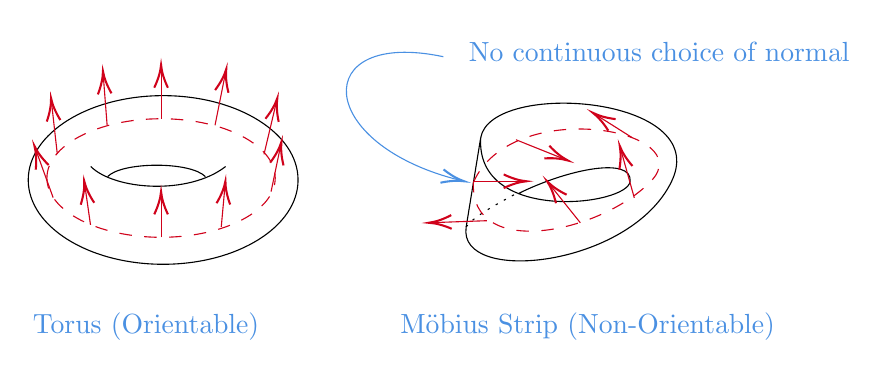
\begin{tikzpicture}[x=0.75pt,y=0.75pt,yscale=-1,xscale=1]
%uncomment if require: \path (0,202); %set diagram left start at 0, and has height of 202

%Curve Lines [id:da05527802912152291] 
\draw    (140.12,72.88) .. controls (151.5,84.25) and (187.25,86.85) .. (205.12,72.88) ;
%Curve Lines [id:da5225555438075742] 
\draw    (195.37,77.75) .. controls (187.9,70.28) and (155.07,70.6) .. (148.25,77.75) ;
%Shape: Ellipse [id:dp3063344683235558] 
\draw   (110,79.38) .. controls (110,56.94) and (139.1,38.75) .. (175,38.75) .. controls (210.9,38.75) and (240,56.94) .. (240,79.38) .. controls (240,101.81) and (210.9,120) .. (175,120) .. controls (139.1,120) and (110,101.81) .. (110,79.38) -- cycle ;
%Straight Lines [id:da6184709043628867] 
\draw [color={rgb, 255:red, 208; green, 2; blue, 27 }  ,draw opacity=1 ]   (223.6,67) -- (229.54,41.95) ;
\draw [shift={(230,40)}, rotate = 103.34] [color={rgb, 255:red, 208; green, 2; blue, 27 }  ,draw opacity=1 ][line width=0.75]    (10.93,-3.29) .. controls (6.95,-1.4) and (3.31,-0.3) .. (0,0) .. controls (3.31,0.3) and (6.95,1.4) .. (10.93,3.29)   ;
%Straight Lines [id:da24851539996932948] 
\draw    (328,59) -- (321,102) ;
%Curve Lines [id:da7319120828999304] 
\draw    (328,59) .. controls (333,31) and (439.8,38.6) .. (420,80) .. controls (400.2,121.4) and (316.6,130.2) .. (321,102) ;
%Curve Lines [id:da955357858158234] 
\draw    (328,59) .. controls (325.4,100.6) and (399,91.8) .. (400,80) .. controls (401,68.2) and (370.6,73.8) .. (346,86) ;
%Curve Lines [id:da1240095272344981] 
\draw  [dash pattern={on 0.84pt off 2.51pt}]  (321,102) .. controls (324.6,97) and (335,91.4) .. (345,86) ;
%Shape: Ellipse [id:dp5049740326726107] 
\draw  [color={rgb, 255:red, 208; green, 2; blue, 27 }  ,draw opacity=1 ][dash pattern={on 4.5pt off 4.5pt}] (119,78.44) .. controls (119,62.66) and (143.62,49.88) .. (174,49.88) .. controls (204.38,49.88) and (229,62.66) .. (229,78.44) .. controls (229,94.21) and (204.38,107) .. (174,107) .. controls (143.62,107) and (119,94.21) .. (119,78.44) -- cycle ;
%Straight Lines [id:da9359578969630631] 
\draw [color={rgb, 255:red, 208; green, 2; blue, 27 }  ,draw opacity=1 ]   (200,53) -- (205.01,27.96) ;
\draw [shift={(205.4,26)}, rotate = 101.31] [color={rgb, 255:red, 208; green, 2; blue, 27 }  ,draw opacity=1 ][line width=0.75]    (10.93,-3.29) .. controls (6.95,-1.4) and (3.31,-0.3) .. (0,0) .. controls (3.31,0.3) and (6.95,1.4) .. (10.93,3.29)   ;
%Straight Lines [id:da3289515902723321] 
\draw [color={rgb, 255:red, 208; green, 2; blue, 27 }  ,draw opacity=1 ]   (174,49.88) -- (174,26) ;
\draw [shift={(174,24)}, rotate = 90] [color={rgb, 255:red, 208; green, 2; blue, 27 }  ,draw opacity=1 ][line width=0.75]    (10.93,-3.29) .. controls (6.95,-1.4) and (3.31,-0.3) .. (0,0) .. controls (3.31,0.3) and (6.95,1.4) .. (10.93,3.29)   ;
%Straight Lines [id:da09641925370320403] 
\draw [color={rgb, 255:red, 208; green, 2; blue, 27 }  ,draw opacity=1 ]   (148,52.88) -- (146.15,28.99) ;
\draw [shift={(146,27)}, rotate = 85.58] [color={rgb, 255:red, 208; green, 2; blue, 27 }  ,draw opacity=1 ][line width=0.75]    (10.93,-3.29) .. controls (6.95,-1.4) and (3.31,-0.3) .. (0,0) .. controls (3.31,0.3) and (6.95,1.4) .. (10.93,3.29)   ;
%Straight Lines [id:da2908901884677755] 
\draw [color={rgb, 255:red, 208; green, 2; blue, 27 }  ,draw opacity=1 ]   (124,66.88) -- (121.22,41.99) ;
\draw [shift={(121,40)}, rotate = 83.63] [color={rgb, 255:red, 208; green, 2; blue, 27 }  ,draw opacity=1 ][line width=0.75]    (10.93,-3.29) .. controls (6.95,-1.4) and (3.31,-0.3) .. (0,0) .. controls (3.31,0.3) and (6.95,1.4) .. (10.93,3.29)   ;
%Straight Lines [id:da23254355767226764] 
\draw [color={rgb, 255:red, 208; green, 2; blue, 27 }  ,draw opacity=1 ]   (122,87.88) -- (113.68,64.88) ;
\draw [shift={(113,63)}, rotate = 70.11] [color={rgb, 255:red, 208; green, 2; blue, 27 }  ,draw opacity=1 ][line width=0.75]    (10.93,-3.29) .. controls (6.95,-1.4) and (3.31,-0.3) .. (0,0) .. controls (3.31,0.3) and (6.95,1.4) .. (10.93,3.29)   ;
%Straight Lines [id:da5510348186397793] 
\draw [color={rgb, 255:red, 208; green, 2; blue, 27 }  ,draw opacity=1 ]   (140,101) -- (137.28,81.98) ;
\draw [shift={(137,80)}, rotate = 81.87] [color={rgb, 255:red, 208; green, 2; blue, 27 }  ,draw opacity=1 ][line width=0.75]    (10.93,-3.29) .. controls (6.95,-1.4) and (3.31,-0.3) .. (0,0) .. controls (3.31,0.3) and (6.95,1.4) .. (10.93,3.29)   ;
%Straight Lines [id:da05975983118898509] 
\draw [color={rgb, 255:red, 208; green, 2; blue, 27 }  ,draw opacity=1 ]   (174,107) -- (174,87) ;
\draw [shift={(174,85)}, rotate = 90] [color={rgb, 255:red, 208; green, 2; blue, 27 }  ,draw opacity=1 ][line width=0.75]    (10.93,-3.29) .. controls (6.95,-1.4) and (3.31,-0.3) .. (0,0) .. controls (3.31,0.3) and (6.95,1.4) .. (10.93,3.29)   ;
%Straight Lines [id:da44294131424364247] 
\draw [color={rgb, 255:red, 208; green, 2; blue, 27 }  ,draw opacity=1 ]   (203,102) -- (204.82,81.99) ;
\draw [shift={(205,80)}, rotate = 95.19] [color={rgb, 255:red, 208; green, 2; blue, 27 }  ,draw opacity=1 ][line width=0.75]    (10.93,-3.29) .. controls (6.95,-1.4) and (3.31,-0.3) .. (0,0) .. controls (3.31,0.3) and (6.95,1.4) .. (10.93,3.29)   ;
%Straight Lines [id:da8437130662647478] 
\draw [color={rgb, 255:red, 208; green, 2; blue, 27 }  ,draw opacity=1 ]   (227,85) -- (231.59,62.96) ;
\draw [shift={(232,61)}, rotate = 101.77] [color={rgb, 255:red, 208; green, 2; blue, 27 }  ,draw opacity=1 ][line width=0.75]    (10.93,-3.29) .. controls (6.95,-1.4) and (3.31,-0.3) .. (0,0) .. controls (3.31,0.3) and (6.95,1.4) .. (10.93,3.29)   ;
%Curve Lines [id:da18056505853386673] 
\draw [color={rgb, 255:red, 208; green, 2; blue, 27 }  ,draw opacity=1 ] [dash pattern={on 4.5pt off 4.5pt}]  (324.5,80.5) .. controls (343,38.6) and (434.2,55) .. (410,80) .. controls (385.8,105) and (322.6,118.2) .. (324.5,80.5) -- cycle ;
%Straight Lines [id:da16920344082056782] 
\draw [color={rgb, 255:red, 208; green, 2; blue, 27 }  ,draw opacity=1 ]   (402,88) -- (395.54,64.93) ;
\draw [shift={(395,63)}, rotate = 74.36] [color={rgb, 255:red, 208; green, 2; blue, 27 }  ,draw opacity=1 ][line width=0.75]    (10.93,-3.29) .. controls (6.95,-1.4) and (3.31,-0.3) .. (0,0) .. controls (3.31,0.3) and (6.95,1.4) .. (10.93,3.29)   ;
%Straight Lines [id:da5162379834614435] 
\draw [color={rgb, 255:red, 208; green, 2; blue, 27 }  ,draw opacity=1 ]   (376,100) -- (361.25,81.56) ;
\draw [shift={(360,80)}, rotate = 51.34] [color={rgb, 255:red, 208; green, 2; blue, 27 }  ,draw opacity=1 ][line width=0.75]    (10.93,-3.29) .. controls (6.95,-1.4) and (3.31,-0.3) .. (0,0) .. controls (3.31,0.3) and (6.95,1.4) .. (10.93,3.29)   ;
%Straight Lines [id:da15822931325348022] 
\draw [color={rgb, 255:red, 208; green, 2; blue, 27 }  ,draw opacity=1 ]   (331,99) -- (305,99.93) ;
\draw [shift={(303,100)}, rotate = 357.95] [color={rgb, 255:red, 208; green, 2; blue, 27 }  ,draw opacity=1 ][line width=0.75]    (10.93,-3.29) .. controls (6.95,-1.4) and (3.31,-0.3) .. (0,0) .. controls (3.31,0.3) and (6.95,1.4) .. (10.93,3.29)   ;
%Straight Lines [id:da3341110759567949] 
\draw [color={rgb, 255:red, 208; green, 2; blue, 27 }  ,draw opacity=1 ]   (325,80) -- (348,80) ;
\draw [shift={(350,80)}, rotate = 180] [color={rgb, 255:red, 208; green, 2; blue, 27 }  ,draw opacity=1 ][line width=0.75]    (10.93,-3.29) .. controls (6.95,-1.4) and (3.31,-0.3) .. (0,0) .. controls (3.31,0.3) and (6.95,1.4) .. (10.93,3.29)   ;
%Straight Lines [id:da17563158134376344] 
\draw [color={rgb, 255:red, 208; green, 2; blue, 27 }  ,draw opacity=1 ]   (345,60) -- (368.14,69.26) ;
\draw [shift={(370,70)}, rotate = 201.8] [color={rgb, 255:red, 208; green, 2; blue, 27 }  ,draw opacity=1 ][line width=0.75]    (10.93,-3.29) .. controls (6.95,-1.4) and (3.31,-0.3) .. (0,0) .. controls (3.31,0.3) and (6.95,1.4) .. (10.93,3.29)   ;
%Straight Lines [id:da5963965638960156] 
\draw [color={rgb, 255:red, 208; green, 2; blue, 27 }  ,draw opacity=1 ]   (401,59) -- (383.69,48.07) ;
\draw [shift={(382,47)}, rotate = 32.28] [color={rgb, 255:red, 208; green, 2; blue, 27 }  ,draw opacity=1 ][line width=0.75]    (10.93,-3.29) .. controls (6.95,-1.4) and (3.31,-0.3) .. (0,0) .. controls (3.31,0.3) and (6.95,1.4) .. (10.93,3.29)   ;
%Curve Lines [id:da24333526890590362] 
\draw [color={rgb, 255:red, 74; green, 144; blue, 226 }  ,draw opacity=1 ]   (310,20) .. controls (245.32,6.27) and (247.31,62.43) .. (318.92,79.74) ;
\draw [shift={(320,80)}, rotate = 193.17] [color={rgb, 255:red, 74; green, 144; blue, 226 }  ,draw opacity=1 ][line width=0.75]    (10.93,-3.29) .. controls (6.95,-1.4) and (3.31,-0.3) .. (0,0) .. controls (3.31,0.3) and (6.95,1.4) .. (10.93,3.29)   ;

% Text Node
\draw (111,142) node [anchor=north west][inner sep=0.75pt]  [color={rgb, 255:red, 74; green, 144; blue, 226 }  ,opacity=1 ] [align=left] {Torus (Orientable)};
% Text Node
\draw (288,142) node [anchor=north west][inner sep=0.75pt]  [color={rgb, 255:red, 74; green, 144; blue, 226 }  ,opacity=1 ] [align=left] {Möbius Strip (Non-Orientable)};
% Text Node
\draw (321,12) node [anchor=north west][inner sep=0.75pt]  [color={rgb, 255:red, 74; green, 144; blue, 226 }  ,opacity=1 ] [align=left] {No continuous choice of normal};


\end{tikzpicture}


\end{center}

\section{Geometry of Surfaces in \texorpdfstring{$\R^3$}{R3}}

\subsection{First Fundamental Form}

Having developed some ways to discuss surfaces particularly in $\R^3$, we are going to start discussing more geometric notions such as length and angles.

Recall that for a curve $\gamma: (a, b) \rightarrow \R^3$, the length of $\gamma$ is given by
$$
L(\gamma) = \int_a^b \norm{\gamma'(t)} \dd t.
$$
Since this is independent of paramterisation\footnote{Feel free to check this}, we can naturally parameterise a curve with respect to arc length (as long as $\gamma'(t) \neq 0$). Now, given a curve on some smooth surface in $\R^3$, we want to find a nice way to compute lengths.

let $\Sigma$ be a smoth surface in $\R^3$, and let $\sigma: V \rightarrow U \subseteq \Sigma$ be an allowable parameterisation. Let $\gamma: (a, b) \rightarrow \R^3$ be smooth and have its image be contained in $U$. Then writing $\gamma(t) = \sigma(u(t), v(t))$, and so $\gamma'(t) = \sigma_u u'(t) + \sigma_v v'(t)$, giving
$$
\norm{\gamma'(t)} = E u'(t)^2 + 2F u'(t) v(t) + Gv'(t)^2,
$$
for functions
$$
E = \langle \sigma_u, \sigma_u\rangle; \quad F = \langle \sigma_u, \sigma_v \rangle = \langle \sigma_v, \sigma_u \rangle; \quad G = \langle \sigma_v, \sigma_v \rangle,
$$
where $\langle \cdot, \cdot \rangle$ is our Euclidean inner product. These values encapsulate the notion of length for our surface.

\begin{definition}[First Fundamental Form]
    The \vocab{first fundamental form} of $\Sigma$ in the parameterisation $\sigma$ is the expression
    $$
    E \dd u^2 + 2F \dd u \dd v + G \dd v^2.
    $$
\end{definition}

Note that if $\gamma$ has image in the image of $\sigma$, then
$$
L(\gamma) = \int_a^b \sqrt{E (u')^2 + 2F u' v' + G(v')^2} \dd t.
$$
With length encapsulated by the first fundamental form, we get a nice way to capture when two surfaces (locally) have the same `geometry' in a \emph{length} sense.

\begin{definition}[Isometric]
    Let $\Sigma, \Sigma'$ be smooth surfaces in $\R^3$. We say that they are \vocab{isometric} if there exists a diffeomorphism $f: \Sigma \rightarrow \Sigma'$ that preserves the length of al curves.
\end{definition}
\begin{definition}[Locally Isometric]
    We say that $\Sigma, \Sigma'$ are \emph{locally isometric} near points $p \in \Sigma$ and $q \in \Sigma'$ if there exists open neighbourhoods $U$ of $p$ and $V$ of $q$ such that $U$ and $V$ are isometric.
\end{definition}
\begin{lemma}
    Smooth surfaces $\Sigma, \Sigma'$ in $\R^3$ are locally isometric near $p \in \Sigma$ and $q \in \Sigma'$ if and only if there exist allowable parameterisations $\sigma: V \rightarrow U \subseteq \Sigma$ and $\sigma': V \rightarrow U' \subseteq \Sigma'$ such that the first fundamental forms are equivalent. 
\end{lemma}
\begin{proof}
    Omitted.
\end{proof}

\subsection{Area}

With length pinned down by the first fundamental form, it's not too hard to pin down area. 

Recall that a parallelogram spanned by two vectors $v, w$ has area $|v \times w| = \langle v, v \rangle \langle w, w \rangle - \langle v, w \rangle^2$. So if we have an allowable parameterisation $\sigma: V \rightarrow U \subseteq \Sigma$ with $\sigma(0) = p$, and consider $\sigma_u, \sigma_v \in T_p \Sigma$, the square of the area of the infinitesimal parallelogram spanned by $\sigma_u, \sigma_v$ is given by
$$
\langle \sigma_u, \sigma_u \rangle \langle \sigma_v, \sigma_v \rangle - \langle \sigma_u, \sigma_v \rangle^2 = EG - F^2.
$$
This gives us a sensible way to define area.

\begin{definition}[Area]
    Let $\Sigma$ be a smooth surface in $\R^3$, and let $\sigma: V \rightarrow U \subseteq \Sigma$ be an allowable parameterisation. Then
    $$
\operatorname{area}(U) = \int_V \sqrt{EG - F^2} \dd u \dd v.
    $$
\end{definition}

\subsection{Second Fundamental Form}


Intuitively, the first fundamental form pins down how length works along our surface. We now, through the second fundamental form, will try to pin down how \emph{curved} our surface is (as an embedding of $\R^3$).

We are (informally) going to look at curvature at a point as measuring how much we deviate from the tangent plane by moving a small amount away from our point.

\begin{center}
    

\tikzset{every picture/.style={line width=0.75pt}} %set default line width to 0.75pt        

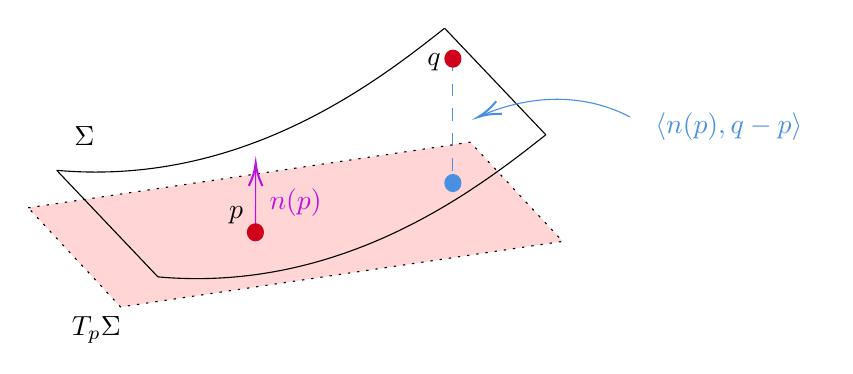
\begin{tikzpicture}[x=0.75pt,y=0.75pt,yscale=-1,xscale=1]
%uncomment if require: \path (0,459); %set diagram left start at 0, and has height of 459

%Shape: Parallelogram [id:dp7900821750552607] 
\draw  [fill={rgb, 255:red, 255; green, 179; blue, 179 }  ,fill opacity=0.55 ][dash pattern={on 0.84pt off 2.51pt}] (6,89.18) -- (218.98,57.58) -- (263.5,105.36) -- (50.51,136.96) -- cycle ;
%Straight Lines [id:da32794339542910955] 
\draw [color={rgb, 255:red, 74; green, 144; blue, 226 }  ,draw opacity=1 ] [dash pattern={on 4.5pt off 4.5pt}]  (210.61,17.34) -- (210.61,77.25) ;
%Straight Lines [id:da9843969307420661] 
\draw    (19.72,71.13) -- (68.48,122.47) ;
%Curve Lines [id:da6590186468140269] 
\draw    (68.48,122.47) .. controls (157.86,130.43) and (222.87,79.69) .. (255.37,54.01) ;
%Curve Lines [id:da12117500145497906] 
\draw    (19.72,71.13) .. controls (109.11,79.09) and (174.11,28.34) .. (206.62,2.67) ;
%Straight Lines [id:da969061893759412] 
\draw    (206.62,2.67) -- (255.37,54.01) ;
%Shape: Ellipse [id:dp3759846798866977] 
\draw  [draw opacity=0][fill={rgb, 255:red, 208; green, 2; blue, 27 }  ,fill opacity=1 ] (206.47,17.34) .. controls (206.47,14.93) and (208.33,12.98) .. (210.61,12.98) .. controls (212.89,12.98) and (214.74,14.93) .. (214.74,17.34) .. controls (214.74,19.75) and (212.89,21.71) .. (210.61,21.71) .. controls (208.33,21.71) and (206.47,19.75) .. (206.47,17.34) -- cycle ;
%Shape: Ellipse [id:dp4473354880432048] 
\draw  [draw opacity=0][fill={rgb, 255:red, 74; green, 144; blue, 226 }  ,fill opacity=1 ] (206.47,77.25) .. controls (206.47,74.84) and (208.33,72.88) .. (210.61,72.88) .. controls (212.89,72.88) and (214.74,74.84) .. (214.74,77.25) .. controls (214.74,79.66) and (212.89,81.61) .. (210.61,81.61) .. controls (208.33,81.61) and (206.47,79.66) .. (206.47,77.25) -- cycle ;
%Straight Lines [id:da32292000427802847] 
\draw [color={rgb, 255:red, 189; green, 16; blue, 224 }  ,draw opacity=1 ]   (115.47,100.99) -- (115.6,69.71) ;
\draw [shift={(115.61,67.71)}, rotate = 90.24] [color={rgb, 255:red, 189; green, 16; blue, 224 }  ,draw opacity=1 ][line width=0.75]    (10.93,-3.29) .. controls (6.95,-1.4) and (3.31,-0.3) .. (0,0) .. controls (3.31,0.3) and (6.95,1.4) .. (10.93,3.29)   ;
%Shape: Ellipse [id:dp3469616434750329] 
\draw  [draw opacity=0][fill={rgb, 255:red, 208; green, 2; blue, 27 }  ,fill opacity=1 ] (111.33,100.99) .. controls (111.33,98.58) and (113.18,96.63) .. (115.47,96.63) .. controls (117.75,96.63) and (119.6,98.58) .. (119.6,100.99) .. controls (119.6,103.4) and (117.75,105.36) .. (115.47,105.36) .. controls (113.18,105.36) and (111.33,103.4) .. (111.33,100.99) -- cycle ;
%Curve Lines [id:da36924394958097206] 
\draw [color={rgb, 255:red, 74; green, 144; blue, 226 }  ,draw opacity=1 ]   (296,45.42) .. controls (271.44,32.74) and (245.33,35.68) .. (224.46,44.71) ;
\draw [shift={(222.87,45.42)}, rotate = 335.61] [color={rgb, 255:red, 74; green, 144; blue, 226 }  ,draw opacity=1 ][line width=0.75]    (10.93,-3.29) .. controls (6.95,-1.4) and (3.31,-0.3) .. (0,0) .. controls (3.31,0.3) and (6.95,1.4) .. (10.93,3.29)   ;

% Text Node
\draw (101.48,87.28) node [anchor=north west][inner sep=0.75pt]  [color={rgb, 255:red, 0; green, 0; blue, 0 }  ,opacity=1 ]  {$p$};
% Text Node
\draw (27,48.81) node [anchor=north west][inner sep=0.75pt]  [color={rgb, 255:red, 0; green, 0; blue, 0 }  ,opacity=1 ]  {$\Sigma $};
% Text Node
\draw (25.76,140.4) node [anchor=north west][inner sep=0.75pt]  [color={rgb, 255:red, 0; green, 0; blue, 0 }  ,opacity=1 ]  {$T_{p} \Sigma $};
% Text Node
\draw (197,13.81) node [anchor=north west][inner sep=0.75pt]  [color={rgb, 255:red, 0; green, 0; blue, 0 }  ,opacity=1 ]  {$q$};
% Text Node
\draw (121,78.81) node [anchor=north west][inner sep=0.75pt]  [color={rgb, 255:red, 189; green, 16; blue, 224 }  ,opacity=1 ]  {$n( p)$};
% Text Node
\draw (297,42) node [anchor=north west][inner sep=0.75pt]  [color={rgb, 255:red, 74; green, 144; blue, 226 }  ,opacity=1 ] [align=left] {\begin{minipage}[lt]{67.96pt}\setlength\topsep{0pt}
\begin{center}
$\displaystyle \langle n( p) ,q-p\rangle $
\end{center}

\end{minipage}};


\end{tikzpicture}

\end{center}

Let $\Sigma$ be a smooth surface in $\R^3$, and let $\sigma: V \rightarrow U \subseteq \Sigma$ be an allowable parameterisation. Consider a point $p = \sigma(u, v)$, and some nearby point $q = \sigma(u + h, v + \ell)$. Then by Taylor's theorem we have
\begin{align*}
\sigma(u + h, v + \ell) &= \sigma(u, v) + h \sigma_u(u, v) + \ell \sigma_v(u, v) \\
&\ + \frac{1}{2}\left(h^2 \sigma_uu(u, v) + 2 h\ell \sigma_{uv}(u, v) + \ell^2 \sigma_{vv}(u, v)\right)\\&\ + O(h^3, \ell^3).
\end{align*}
Recalling that the tangent plane is given by $T_p\Sigma = \operatorname{span}\{\sigma_u, \sigma_v\}$, we get the perpendicular distance from $q = \sigma(u + h, v+\ell)$ to the affine tangent plane $T_p\Sigma + p$ is given by
\begin{align*}
    \langle n, \sigma(u + h, v + \ell) - \sigma(u, v)\rangle &= \frac{1}{2}\left(\langle n, \sigma_{uu} \rangle h^2 + 2 \langle h, \sigma_{uv}\rangle h \ell + \langle n, \sigma_{vv} \rangle \ell^2\right)\\&\  + O(h^3, l^3). 
\end{align*}
and so we can see that these inner products give us this difference. This inspires our definition of the second fundamental form.

\begin{definition}[Second Fundamental Form]
    The \vocab{second fundamental form} of $\Sigma$ in the allowable parameterisation $\sigma$ is
    $$
    L \dd u^2 + 2M \dd u \dd v + N \dd v^2
    $$
    where $L = \langle n, \sigma_{uu} \rangle$, $M =  \langle n, \sigma_{uv} \rangle$, and $N = \langle n, \sigma_{vv} \rangle$, and $n$ is the unit normal given by $n = \frac{\sigma_u \times \sigma_v}{\norm{\sigma_u \times \sigma_v}}$.
\end{definition}

We will say more about how this relates to curvature in the coming sections. It's good to know (but not proven in this course) that the two fundamental forms completely determine a smooth oriented connected surface in $\R^3$, up to rigid motion. This is the \emph{fundamental theorem of surfaces in $\R^3$}.

\subsection{The Gauss Map and Curvature}

We are now going to define what our notion of curvature actually is. This is done using the \emph{Gauss map}.

\begin{definition}[Gauss Map]
    Let $\Sigma$ be a smooth oriented surface in $\R^3$. The \vocab{Gauss map} $n : \Sigma \rightarrow S^2$ is the map $p \mapsto n(p)$, where the normal vector is normalised and hence lies in the unit sphere.
\end{definition}

% \begin{lemma}
%     The Gauss map is smooth.
% \end{lemma}

% \begin{proof}
%     Let $p \in \Sigma$ and let $\sigma: V \rightarrow U \subseteq \Sigma$ with $p \in U$ be allowable and compatible with our chosen orientation. Then
%     $$
%     n(p) = \frac{\sigma_u \times \sigma_v}{\norm{\sigma_u \times \sigma_v}}.
%     $$
%     Since $\sigma$ is allowable, the denominator is non-vanishing and hence $n(p)$ is smooth as required.
% \end{proof}

\begin{definition}[Gauss Curvature]
    Let $\Sigma$ be a smooth surface in $\R^3$. The \vocab{Gauss curvature $\kappa$} is $\kappa: \Sigma \rightarrow \R$ given by
    $$
    \kappa(p) = \det \left(\left.Dn\right|_p\right)
    $$
\end{definition}

We note that this is smooth since the Gauss map is smooth\footnote{Follows by writing down an expression for $n(p)$ and noting that it's the composition of smooth functions.} and is also always well defined even for non-orientable $\Sigma$, as $\Sigma$ is always locally orientable.

We can compute $\kappa$ by using the first and second fundamental forms, but it will require looking at these from a different perspective.

\subsubsection*{A Different Perspective on the Fundamental Forms}

The first fundamental form specifies 

We can compute what $\kappa$ is exactly.
{\color{red} TODO: FILL IN THE DETAILS}. And we arrive at
$$
\kappa = \frac{LN - M^2}{EG - F^2}.
$$


\begin{definition}
    A smooth surface in $\R^3$ with vanishing gauss curvature everywhere is called flat.
\end{definition}

\begin{definition}
    Let $\Sigma$ be a smooth surface in $\R^3$, and let $p \in \Sigma$. We say that
    \begin{enumerate}[label=(\roman*)]
        \item \vocab{elliptic} if $\kappa(p) > 0$;
        \item \vocab{hyperbolic} if $\kappa(p) < 0$;
        \item \vocab{parabolic} if $\kappa(p) = 0$.
    \end{enumerate}
\end{definition}

\begin{lemma}
    In sufficiently small nbhd of elliptic point, surface lies entirely to one side.
\end{lemma}
\begin{theorem}
    Compact smooth surface has elliptic point.
\end{theorem}

Now an interpretation of Gauss curvature. 

\begin{theorem}
    Let $\Sigma$ be a smooth surface in $\R^3$, and let $p \in \Sigma$ such that $\kappa(p) \neq 0$. Let $U$ be an open neighborhood of $p$, and a decreasing sequence $A_i \subseteq U$ of neighborhoods that `shrink to $p$' in the sense that for all $\varepsilon > 0$, $A_i \subseteq B(p, \varepsilon)$ for sufficiently large $i$. Then,
    $$
    |\kappa(p) | = \lim_{i \to \infty} \frac{\operatorname{area}_{S^2}(n(A_i))}{\operatorname{area}_\Sigma (A_i)}.
    $$
\end{theorem}
Informally, Gauss curvature is an infinitesimal measure of how much the Gauss map $n$ distorts area.

\begin{theorem}[Theorema Egregium]
    The gauss curvature is isometry invariant.
\end{theorem}

\begin{theorem}[Gauss-Bonnet]
    If $\Sigma$ is a compact smooth surface in $\R^3$, then
    $$
    \int_{\Sigma} \kappa \dd A_\Sigma = 2 \pi \chi(\Sigma).
    $$
\end{theorem}
% Let $\sigma: V \rightarrow U \subseteq \Sigma$ be an allowable parametrization, and let $p \in U$. Then noting that $\langle n, n\rangle = 0$, differentiating gives $\langle n, n_u \rangle = \langle n, n_v \rangle = 0$. Then since $\{\sigma_u, \sigma_v, n\}$ forms a basis, there's some $a, b, c, d$ such that
% $$
% n_u = a \sigma_u + b \sigma_v, \quad \text{and} \quad n_v = c \sigma_u + d \sigma_v.
% $$
% Now we also know that $\langle n, \sigma_u \rangle = 0$, and differentiating this gives $\langle n_u, \sigma_u\rangle + \langle n, \sigma_{uu} \rangle = 0$, that is, $\langle n_u, \sigma_u\rangle = -L$. Continuing on like this, we get
% $$
% -L = \langle n_u, \sigma_u \rangle, \quad -N = \langle n_v, \sigma_v \rangle, \quad -M = \langle n_v, \sigma_u \rangle.
% $$

% Other POV: FFF is bilinear form $I: T_p\Sigma \rightarrow T_p \Sigma$, so $I(v, w) = \langle v, w \rangle$. SFF is as before, and $I = (D\sigma)^T D\sigma$. $II = -(Dn)^T D\sigma$

% \section{Some Topological Surfaces}

% \subsection{}

% \appendix

% \section{The Inverse and Implicit Function Theorems}

% Test

\section{Geodesics}

\subsection{Definitions}

We are now going to discuss a particular geometric phenomena, \emph{geodesics}, which are curves with (in some sense) are the shortest path between points.

\begin{definition}[Energy]
    The \vocab{energy} of a curve $\gamma$ is given by 
    $$E(\gamma) = \int_a^b \norm{\gamma'(t)}^2 \dd t.$$
\end{definition}

\begin{definition}[One-Parameter Variation]
    Let $\gamma: [a, b] \rightarrow \Sigma$, where $\Sigma$ is a smooth surface in $\R^3$. A \vocab{one-parameter variation} (with fixed-endpoints) of $\gamma$ is a smooth map $\Gamma: (-\varepsilon, \varepsilon) \times [a, b] \rightarrow \Sigma$, such that if $\gamma_s = \gamma(s, \cdot)$, then $\gamma_0(t) = \gamma(t)$ and $\gamma_s(a)$ and $\gamma_s(b)$ are independent of $s$.
\end{definition}

\begin{definition}[Geodesic]
    A smooth curve $\gamma: [a, b] \rightarrow \Sigma$ is a \vocab{geodesic} if\footnote{Alternatively, $\gamma$ is a critical point of the energy functional on curves from $\gamma(a)$ to $\gamma(b)$.}, for every variation $(\gamma_s)$ of $\gamma$ with fixed endpoints, we have $\left.\frac{\dd}{\dd s}\right|_{s = 0} E(\gamma_s) = 0$.
\end{definition}

\subsection{The Geodesic Equations}

So how do we actually find geodesics? It turns out to be \emph{relatively} easy, using the geodesic equations.

Suppose we have some curve $\gamma$ with image contained in an allowable parameterisation $\sigma$. Then for sufficiently small $s$, we can write $\gamma_s(t) = \sigma(u(s, t), v(s, t))$. 
Now let the first fundamental form with respect to $\sigma$ be
$$
E \dd u ^2 + 2F \dd u \dd v + G \dd v^2.
$$
Then by definition,
$$
E(\gamma_s) = \int_a^b E \dot{u}^2 + 2F \dot{u} \dot{v} + G \dot{v}^2 \dd t.
$$
Differentiating under the integral sign and integrating by parts, we get
$$
\left.\frac{\dd}{\dd s} E(\gamma_s) \right|_{s = 0} = \left.\int_a^b A \frac{\partial u}{\partial s} + B \frac{\partial v}{\partial s} \dd t \right|_{s = 0}
$$
where
\begin{align*}
    A &= E_u \dot{u}^2 + 2F_u \dot{u} \dot{v} + G_u \dot{v}^2 - 2 \frac{\dd}{\dd t} (E \dot{u} + F \dot{v}) \\
    B &= E_v \dot{u}^2 + 2F_v \dot{u} \dot{v} + G_v \dot{v}^2 - 2 \frac{\dd}{\dd t}(F \dot{u} + G\dot{v})
\end{align*}
These give us the \emph{geodesic equations}.

\begin{theorem}[Geodesic Equations]
    A smooth curve $\gamma(t) = \sigma(u(t), v(t))$ is a geodesic if and only if it satisfies the geodesic equations
    \begin{align*}
        \frac{\dd}{\dd t} (E \dot{u} + F \dot{v}) &= \frac{
        E_u \dot{u}^2 + 2F_u \dot{u} \dot{v} + G_u \dot{v}^2}{2} \\
        \frac{\dd}{\dd t}(F \dot{u} + G\dot{v})  &= \frac{E_v \dot{u}^2 + 2F_v \dot{u} \dot{v} + G_v \dot{v}^2}{2}
    \end{align*}
\end{theorem}

Unlike length, energy is sensitive to reparameterisation, but Cauchy-Schwarz gives us that $L(\gamma)^2 \leq E(\gamma) (b - a)$, with equality if and only if $\gamma$ is parameterized proportional to arc length.

\begin{corollary}
    If $\gamma$ has constant speed and locally minimizes length, then it is a geodesic. Further, if $\gamma$ minimizes energy globally, then it minimizes length globally and is parameterized with constant speed.
\end{corollary}

For some examples, the geodesics in the plane consist of straight lines, and the geodesics in the sphere consist of the curves of intersection between the sphere and planes through the origin.

In $\R^2$, the geodesics are not just locally shortest but they are also locally straightest. We would intuitively expect this to hold on other surfaces too. That is, we would expect the change in the tangent vector to be as small as possible subject to the constraint that we lie on the surface.

\begin{theorem}
    Let $\Sigma$ be a smooth surface in $\R^3$. A smooth curve $\gamma:[a, b] \rightarrow \Sigma$ is a geodesic if and only if $\ddot{\gamma}(t)$ is everywhere normal to the surface $\Sigma$.
\end{theorem}
\begin{proof}
    Omitted.
\end{proof}

\subsection{Surfaces of Revolution}

One common surface we come across is a surface of revolution, where we rotate say $\eta(u) = (f(u), 0, g(u))$ where $\nu$ is smooth and injective and $f(u)> 0$ about the $z$ axis.

\begin{definition}
A circle obtained by rotating a point of $\eta$ is called a \vocab{parallel}. A curve obtained by rotating $\eta$ itself by a fixed angle about the $z$-axis is a \vocab{meridian}.
\end{definition}

A plane in $\R^3$ containing the $z$-axis is a plane of symmetry, hence meridians are geodesics\footnote{\color{red} DETAIL HERE!}. Not all parallels are geodesics however.

\begin{lemma}
    A parallel given by $u = u_-0$ is a geodesic when parameterised at constant speed if and only if $f'(u_0) = 0$.
\end{lemma}
\begin{proof}
    Omitted.
\end{proof}

Consider a curve $\gamma(t)$ on $\Sigma$, making an angle $\theta$ with a parallel of radius $\rho = f$.

\begin{theorem}[Clairaut's Relation]
    If $\gamma$ is a geodesic, then $\rho \cos \theta$ is constant along $\gamma$.
\end{theorem}

\subsection{Surfaces of Constant Curvature}

Our result looks like this:

\begin{proposition}
    Let $\Sigma$ be a smooth surface in $\R^3$. Then,
    \begin{enumerate}[label=(\roman*)]
        \item If $\kappa \equiv 0$, then $\Sigma$ is locally isometric to $(\R^2, \dd u^2 + \dd v^2)$
        \item If $\kappa \equiv 1$, then $\Sigma$ is locally isometric to $(S^2, \dd u^2 + \cos^2 u  \dd v^2)$.
    \end{enumerate}
\end{proposition}

\subsection{Riemannian Metrics}

\subsection{The Length Metric}

So far, the geometry of our surfaces has been induced by the space that surface has been embed in (which has so far been $\R^3$). Of course, it's possible to do geometry on surfaces that do not arise in this way. 
One way of specifying the geometry of a surface is with a \emph{Riemannian metric}.

\begin{definition}[Riemannian Metric]
    Let $V \subseteq \R^2$ be an open set. An (abstract) \vocab{Riemannian metric} is a smooth map from $V$ to the set of positive definite symmetric billinear forms, given by
    $$
    v \mapsto \begin{pmatrix}
        E(v) & F(v) \\
        F(v) & G(v)
    \end{pmatrix},
    $$
    such that $E, G, EG - F^2 > 0$.
\end{definition}

If $v$ is a vector at $p \in C$, we can compute its infinitesmal length by
$$
\norm{v}^2 = v^\top \begin{pmatrix}
    E(v) & F(v) \\ F(v) & G(v)
\end{pmatrix} v.
$$
So, if $\gamma: [a, b] \rightarrow V$ is smooth,
$$
L(\gamma) = \int_a^b \sqrt{E \dot{u}^2 + 2F \dot{u}\dot{v} + G \dot{v}^2} \dd t,
$$
where $\gamma(t) = (u(t), v(t))$.

% \section{Hyperbolic Geometry}

% \subsection{The Poincaré Disk}

% Test

\end{document}
